% This version of CVPR template is provided by Ming-Ming Cheng.
% Please leave an issue if you found a bug:
% https://github.com/MCG-NKU/CVPR_Template.

\documentclass[final]{cvpr}

\usepackage{times}
\usepackage{epsfig}
\usepackage{graphicx}
\usepackage{amsmath}
\usepackage{amssymb}
\usepackage[french]{babel}
\usepackage[utf8]{inputenc}
\usepackage{subcaption}
\captionsetup{compatibility=false}
\usepackage{array}
\usepackage{booktabs}
\usepackage{float}
\usepackage{footnote}
% Include other packages here, before hyperref.

% If you comment hyperref and then uncomment it, you should delete
% egpaper.aux before re-running latex.  (Or just hit 'q' on the first latex
% run, let it finish, and you should be clear).
\usepackage[pagebackref=true,breaklinks=true,colorlinks,bookmarks=false]{hyperref}


\def\cvprPaperID{****} % *** Enter the CVPR Paper ID here
\def\confYear{CVPR 2021}
%\setcounter{page}{4321} % For final version only


\begin{document}

%%%%%%%%% TITLE
\title{Sign Language Translation from Video to Text}

\author{Marius \textsc{Schmidt-Mengin}\\
	École des Ponts ParisTech\\
	{\tt\small marius.schmidt.mengin@gmail.com}
% For a paper whose authors are all at the same institution,
% omit the following lines up until the closing ``}''.
% Additional authors and addresses can be added with ``\and'',
% just like the second author.
% To save space, use either the email address or home page, not both
\and
Clément \textsc{Grisi}\\
École des Ponts ParisTech\\
{\tt\small grisi.clement@gmail.com}
}

\maketitle


\begin{abstract}
	Sign Language Transformers \cite{neccam} leverage a Transformer-based encoder-decoder architecture with intermediate gloss supervision to jointly learn continuous sign language recognition and translation. We investigate two avenues for improving the results presented in \cite{neccam}. First, we slightly modify the Sign Language Transformers pipeline by replacing the 2D CNN backbone with a 3D CNN, better suited for processing videos. We experiment with self-supervised techniques to train this new backbone. Then, we train the Transformer-based model with additional human keypoint inputs. Although our experiments weren't conclusive, we still believe that the ideas we explored could lead to improvements in sign language translation.
	
\end{abstract}

\section{Introduction}
According to the World Health Organization, over 5\% of the world’s population -- around 466 million people – are deaf or suffer from disabling hearing loss \cite{WHO}. For many of these individuals, sign language is their primary mean of communication. Despite widespread misconceptions, sign language has its own set of linguistic rules and does not translate the spoken languages word by word. Hence, there is a need for systems to translate sign languages to spoken languages.

\paragraph{Sign Language Translation}Sign language translation is a very challenging task and has been an active field of
research for the past two decades. Most of the research conducted to date has focused on sign language recognition (SLR), that is recognizing the sequence of sign glosses \footnote{sign glosses are spoken language words matching the meaning of signs}, ignoring the linguistic properties of the sign language and assuming that there is a one-to-one mapping to spoken words. Recent advances have tried to tackle sign language translation (SLT), that is the full mapping from signs to spoken words.
Given the complexity of translating sign language video to spoken language sentences in an end-to-end manner (Sign2Text), people have introduced intermediate subtasks to bridge the gap between sign language recognition -- recognizing glosses -- and full translation. A combination of these subtasks, the Sign2Gloss2Text approach, used to be state-of-the-art. It consists in training a Sign2Gloss model to extract gloss sequences from sign language videos, which are then used to solve the translation task as a text-to-text problem by separately training a Gloss2Text model. However, the mid-level gloss representation introduces an information bottleneck. Joint learning of continuous sign language recognition and translation (Sign2(Gloss+Text)), was designed to overcome this bottleneck. We evaluate our approach on the recently released PHOENIX-2014T dataset \cite{phoenix}, which contains sign language videos with gloss annotations and text translations.
\paragraph{Sign Language Transformers}
Introduced in \cite{neccam}, this architecture combines gloss prediction and text translation in a joint model. First, an embeddings is obtained for each frame with a pre-trained CNN. The encoder-decoder transformer is then trained (1) to predict the glosses from the outputs of the encoder with a CTC loss and (2) to predict the translation autoregressively.

%-------------------------------------------------------------------------
\section{Video Representations}
\subsection{Spatial Embeddings}

In Sign Language Transformers \cite{neccam}, the spatial embeddings are extracted with a pre-trained 2D CNN. Notably, the 2D CNN they use for their experiments is an Inception network that was pre-trained on sign language recognition \cite{hmm}. The authors \cite{neccam} showed that this is crucial to achieve good performance, as embeddings extrated with an EfficientNet \cite{effnet} pre-trained on ImageNet are substentially worse on the Sign2Gloss task (the reported WER is almost halved).
It is worth noting that this 2D CNN feature extractor is not trained jointly with the Sign Language Transformer. In the following, these embeddings are referred to as \textit{baseline} embeddings.
\subsection{Spatio-Temporal Embeddings}
We investigate replacing the 2D CNN by a 3D CNN. Our goal is to pre-train this 3D CNN to extract good representations of sign language videos for the Sign2Text task. Training it end-to-end with the Sign Language Transformer is difficult because this requires a lot of GPU memory. Indeed, the input videos can have many frames (up to 475 in the PHOENIX-2014T \cite{phoenix} dataset) and cannot easily be split into multiple parts since they are paired with a sentence. In our experiments, on a single GPU, even a batch size of 1 did not allow us to train with videos of more than 384 frames. Although one could try to reduce the framerate, we prefer to experiment with techniques that do not require textual targets. We experiment with several self-supervised pre-training tasks.
\subsection{Self-Supervised Learning of Video Representations}
Recently, there has been a growing interest in self-supervised learning because it allows to leverage large amounts of unlabeled data. Multiple approaches have been developped for self-supervised learning from videos. We explore two of them: predicting whether a video is played forward or backward \cite{arrow} and predicting the order of shuffled clips \cite{vcop}. Other approaches include learning from temporaly modified videos \cite{playback-rate, pace, temp-trans}, learning to predict the future \cite{pred-coding} and contrastive learning \cite{contrast, bert-video}.
\paragraph{Learning from the Arrow of Time}
It has been shown \cite{arrow} that learning to predict whether a video clip is played forward or backward can be useful to learn good representations of videos. Our intuition tells us that this task may be particularly well adapted for learning high-level representations of sign language videos since it is very hard to solve for humans that do not know sign language.
\paragraph{Predicting the Order of Shuffled Clips}
The goal of this task is to predict the order of different clips in a video. First, 3 non-overlapping clips are extracted from a video. From 6 possible permutation, one is chosen randomly. Each clip is passed through a 3D CNN and average-pooled to a feature vector. The feature vectors of all clips are concatenated and passed through a 2-layer MLP-like neural network, which predicts the permutation of the clips. Intuitively, only a high-level understanding of the videos allows to predict the order of non-overlapping clips.
\subsection{Human Keypoint Estimation}
\subsubsection{Modeling the Body Pose}
Sign language being visual, signers rely on multiple complementary channels to convey information. These can be grouped into two main categories: manual and non-manual features. Manual features mainly correspond to the hand shape and its motion through time. Although these are often considered as the governing part of the sign morphology, they alone do not enclose the full context of the conveyed information. To give clarity, add precisions and nuance their words, signers often use non-manual features, such as facial expressions, mouth gesture and body pose. This motivates our work to investigate whether explicitly modelling the body pose (hands, face, upper body) could benefit neural sign language translation.
\subsubsection{Body Keypoints as Additional Inputs}
In order to extract 2D and 3D body keypoints, we apply a pre-trained version of DOPE \cite{dope} to each frame in the PHOENIX-2014T dataset (Figure \ref{fig:2d_3d}). We slighltly modify the code provided by the authors by adding average and max-pooling layers on top of the ResNet50 backbone. We also experiment with argmax pooling, where we retain the $x$ and $y$ indices of the maximum of each feature map. In total, we have access to three pooled embeddings ($1024$-dim avg- and max-pooled embeddings, $2048$-dim argmax-pooled embeddings) as well as 2D and 3D whole-body keypoints (face: $84$ points, hands: $21$ points, body: $13$ points) for each frame in the PHOENIX-2014T dataset. We normalize the 2D keypoints by substracting the mean and dividing by the standard deviation of the corresponding body part. 3D keypoints are between $0$ and $1$ hence we don't try to normalize them further. In order to assess whether or not these pose estimation features benefit sign language translation, we feed them as additional inputs to the Sign Language Transformer by simply concatenating them with the baseline embeddings.

\begin{figure}[h]
	\begin{subfigure}[h]{0.5\linewidth}
		\centering
			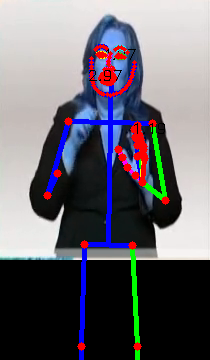
\includegraphics[height=5.5cm]{fig/toy_DOPE_v1_0_0_2d.png}
	\end{subfigure}\hfill
	\begin{subfigure}[]{0.5\linewidth}
		\centering
		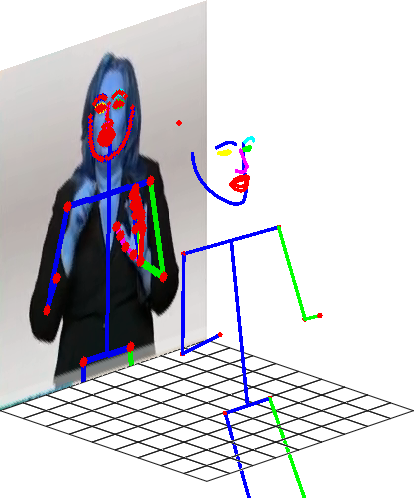
\includegraphics[height=5.5cm]{fig/toy_DOPE_v1_0_0_3d_cropped.png}
	\end{subfigure}
	\caption{2D \& 3D Keypoints on PHOENIX-2014T}
	\label{fig:2d_3d}
\end{figure}

\section{Experiments}
\subsection{Implementation}

To have more flexibility, we re-implement\footnote{\url{https://github.com/marius-sm/sign_language_translation}} Sign Language Transformers \cite{neccam} using Pytorch and HuggingFace transformers \cite{huggingface}. In all our experiments, we use a R(2+1)D \cite{r2plus1} pre-trained on the Kinetics-400 \cite{kinetics} dataset from the Torchvision library as 3D feature extractor. The last convolutional layer produces 512 channels. Whenever necessary, we average-pool those features to produce embeddings. To save training time and reduce GPU memory usage, we downsample the videos to a resolution of $130\times105$ pixels.

To learn the arrow of time, we use clips of 8 frames and train with a batch size of 32. For clip order prediction, we extract 8 clips from each video with intervals of 8 frames and train with a batch size of 8. We optimize both networks with Adam and a low learning rate of $10^{-5}$ to avoid destroying the Kinetics-400 features.

Once trained, we use these networks to extract the embeddings from all videos. As the videos have significantly more than 8 frames,  extracting the embeddings of a video in a single pass results in a strong train/test discrepancy. To adress this issue, we instead subdivide each video in chunks of 8 frames and extract the embedding of each chunk independently.
\subsection{Qualitative Assessments of Embeddings}
After pooling the features along spatial dimensions, we obtain a sequence of spatial embeddings
$$f_t, t\in[1, ..., \tilde{T}]$$
where $\tilde{T}\leq T$ ($T$ is the number of frames of the input video). For a 2D CNN, $T=\tilde{T}$, whereas R(2+1)D has a temporal stride of $8$, resulting in $\tilde{T} = \lceil T/8 \rceil$.
To assess the quality of our embeddings, we visualize their cosine similarities. Given two videos $v^1$ and $v^2$ and their spatial embeddings sequences $f_t^1, t\in\{1, ..., \tilde{T}^1\}$ and $f_u^2, u\in \{1, ...,  \tilde{T}^2\}$, we compute the matrices $A$ and $B$ defined by
$$A_{tt'} = \frac{{f_t^1}^\intercal f_{t'}^1}{\lVert f_t^1 \rVert \lVert f_{t'}^1 \rVert}, \quad\forall t, t' \in\{1, ..., \tilde{T}^1\}$$
$$B_{tu} = \frac{{f_t^1}^\intercal f_u^2}{\lVert f_t^1 \rVert \lVert f_u^2 \rVert}, \quad \forall t \in\{1, ..., \tilde{T}^1\}, u \in\{1, ..., \tilde{T}^2\}$$
That is, we compare the embeddings of a given video with the other embeddings of the same video (matrix $A$) and with the embeddings of another video (matrix $B$). Intuitively, we want 
(1) matrix $A$ to look like a diagonal matrix, where temporaly close frames have similar embeddings, but frames that are far appart have disimilar embeddings, so that there is enough information to recover the translation and (2) matrix $B$ to not have many values close to $1$ as two different videos probably don't translate to related sentences.


\begin{figure}[t]
	\begin{subfigure}[t]{0.5\linewidth}
		\centering\captionsetup{width=.9\linewidth, justification=raggedright}
		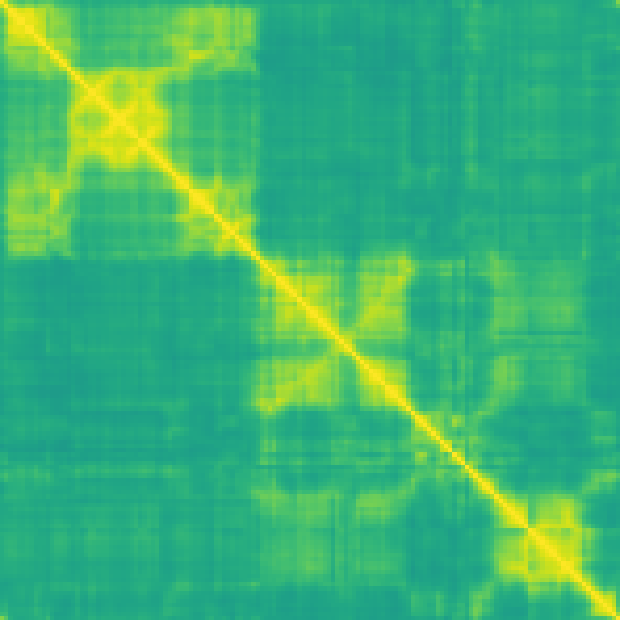
\includegraphics[height=1.8cm]{fig/matrices/a_2d}
		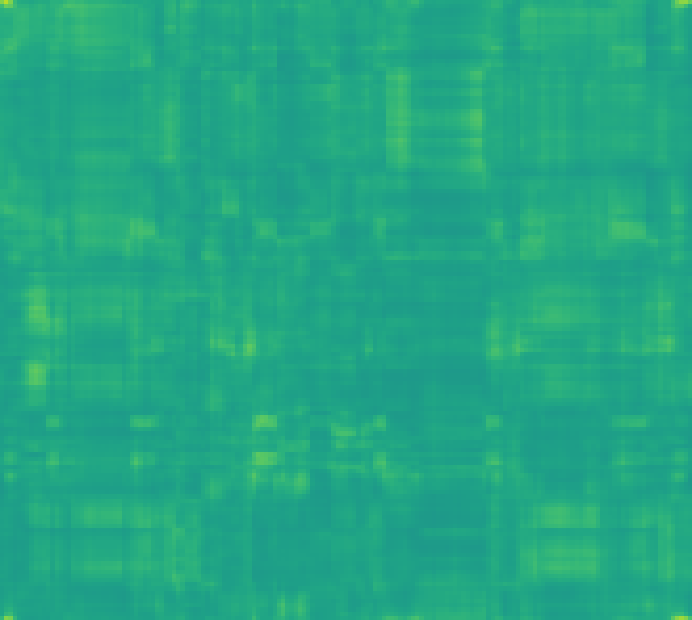
\includegraphics[height=1.8cm]{fig/matrices/b_2d}
		\vspace{-0.1\baselineskip}
		\caption{\centering Inception pre-trained on sign language recognition}
	\end{subfigure}\hfill
	\begin{subfigure}[t]{0.5\linewidth}
		\centering\captionsetup{width=.9\linewidth, justification=raggedright}
		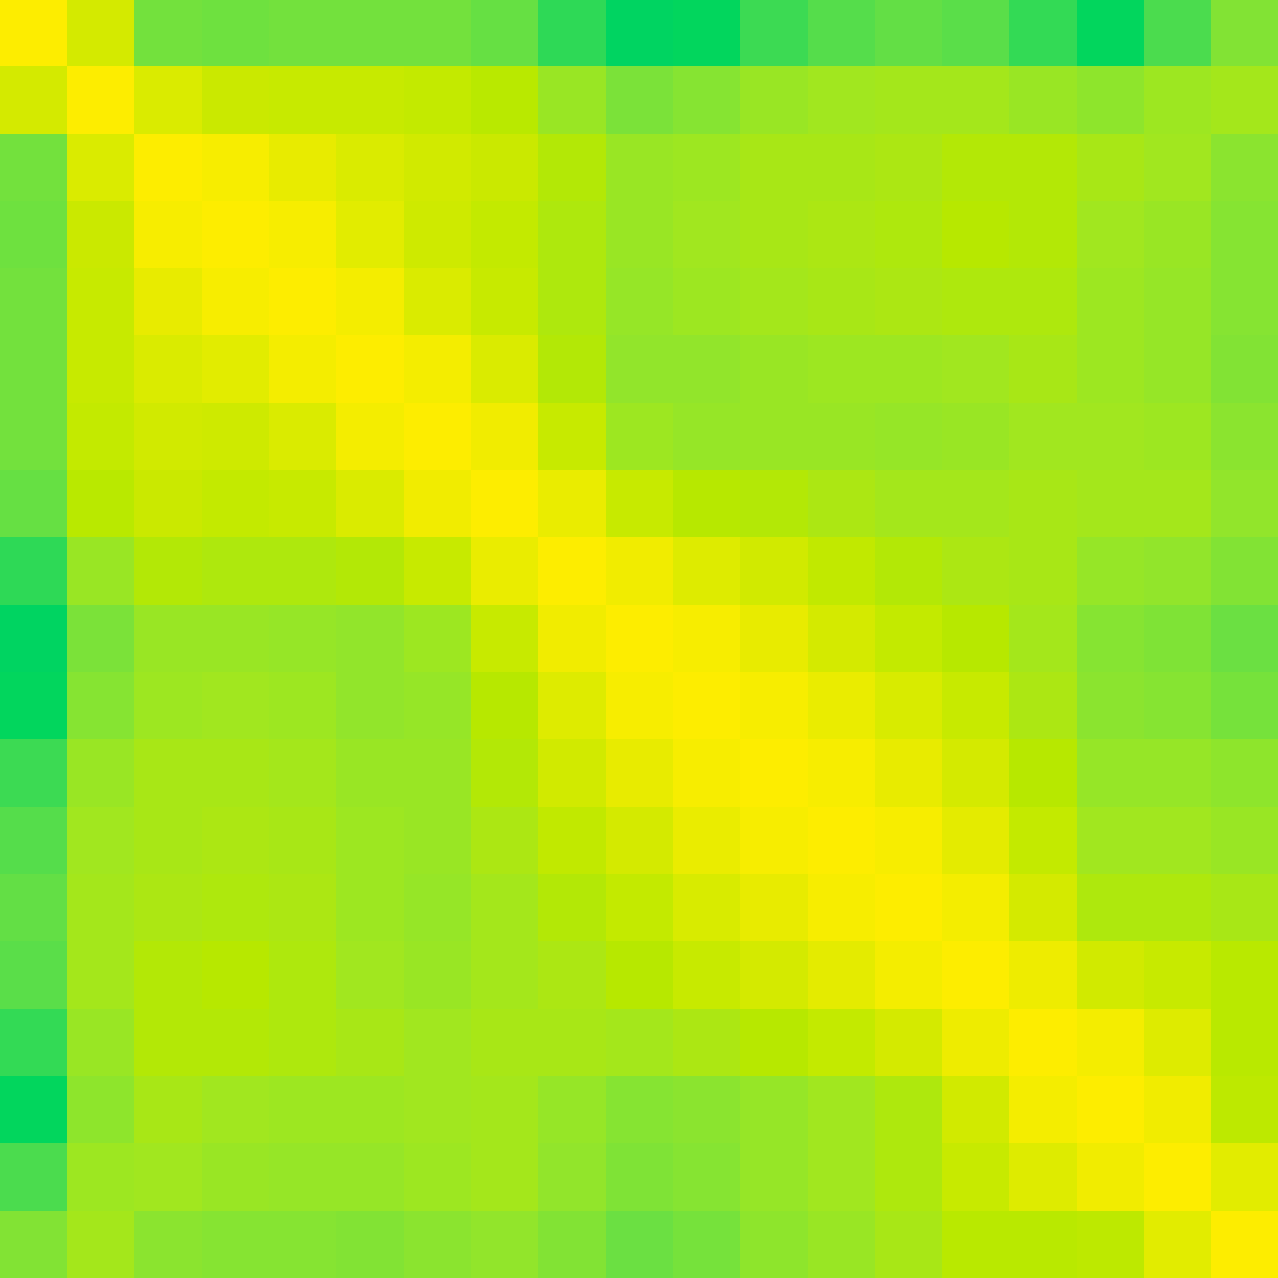
\includegraphics[height=1.8cm]{fig/matrices/a_kinetics}
		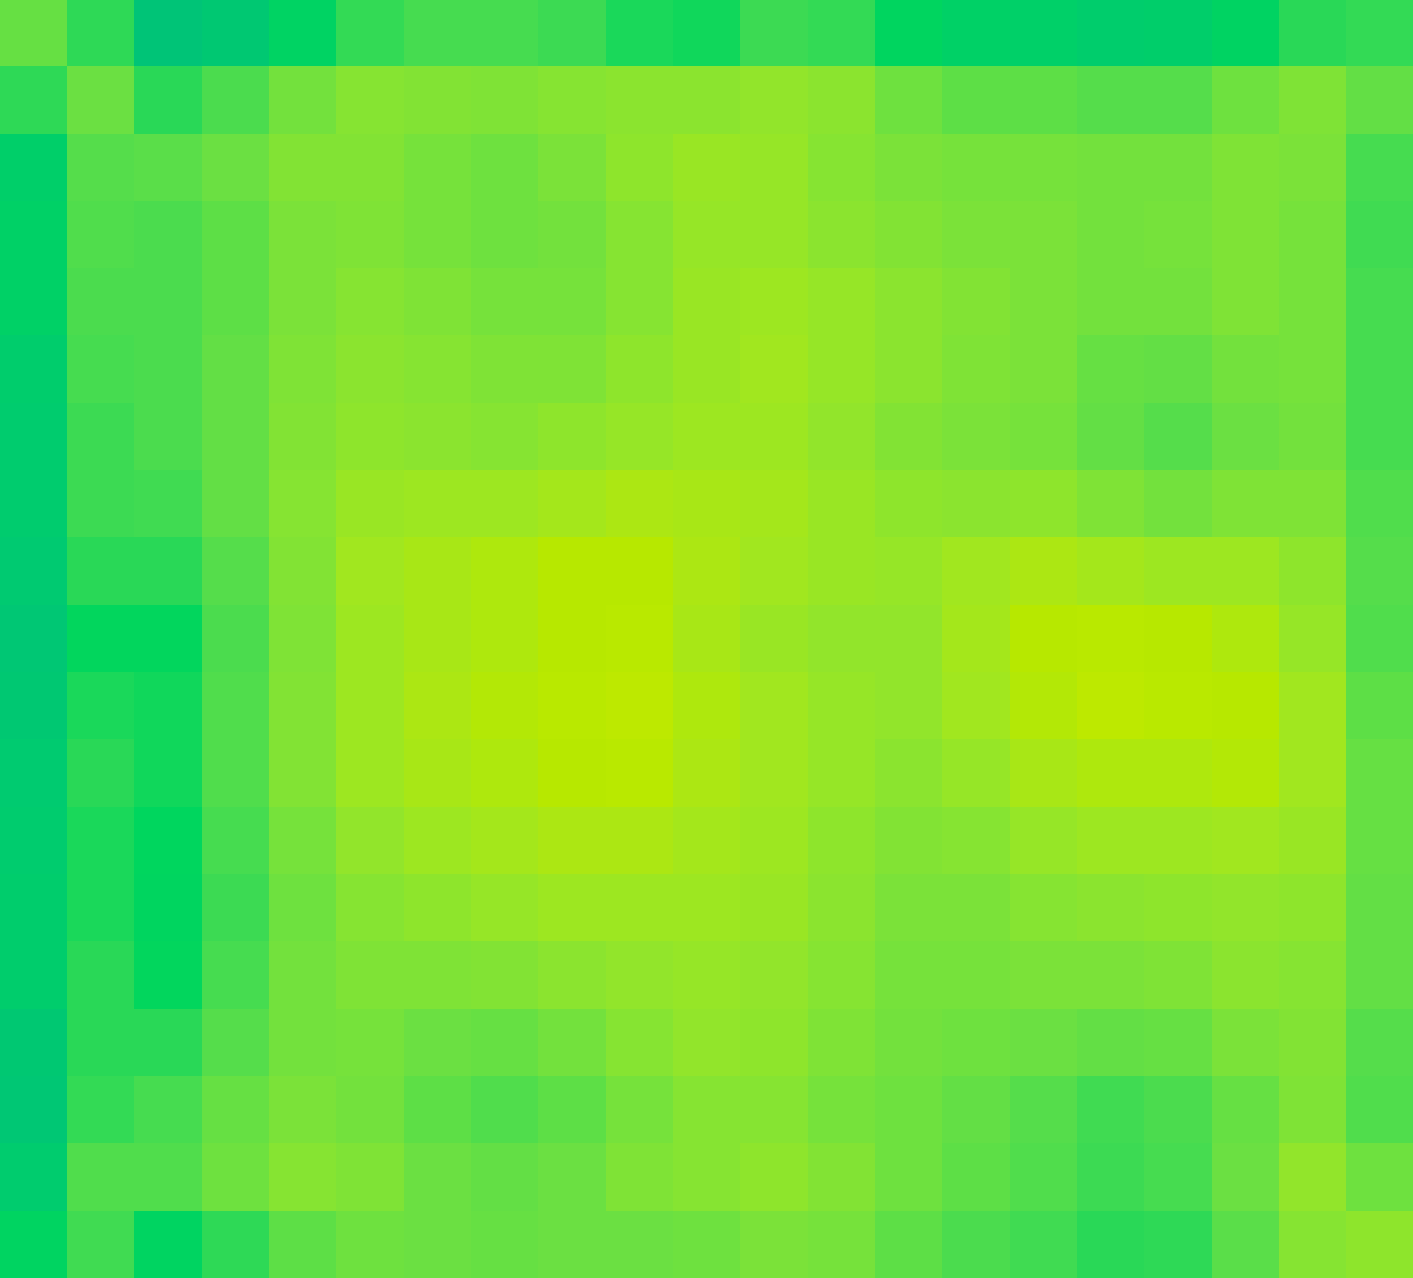
\includegraphics[height=1.8cm]{fig/matrices/b_kinetics}
		\vspace{-0.1\baselineskip}
		\caption{\centering R(2+1)D pre-trained on Kinetics-400}
	\end{subfigure}
	\par\medskip
	\begin{subfigure}[t]{0.5\linewidth}
		\centering\captionsetup{width=.9\linewidth, justification=raggedright}
		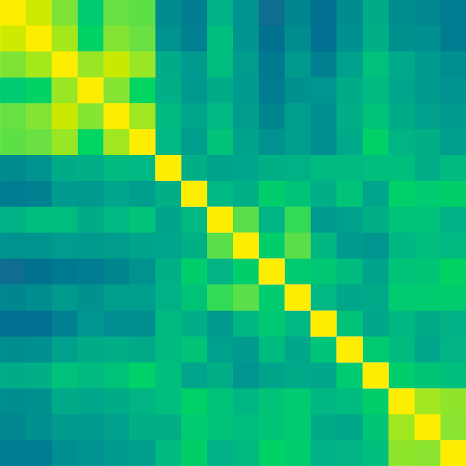
\includegraphics[height=1.8cm]{fig/matrices/a_tarrow}
		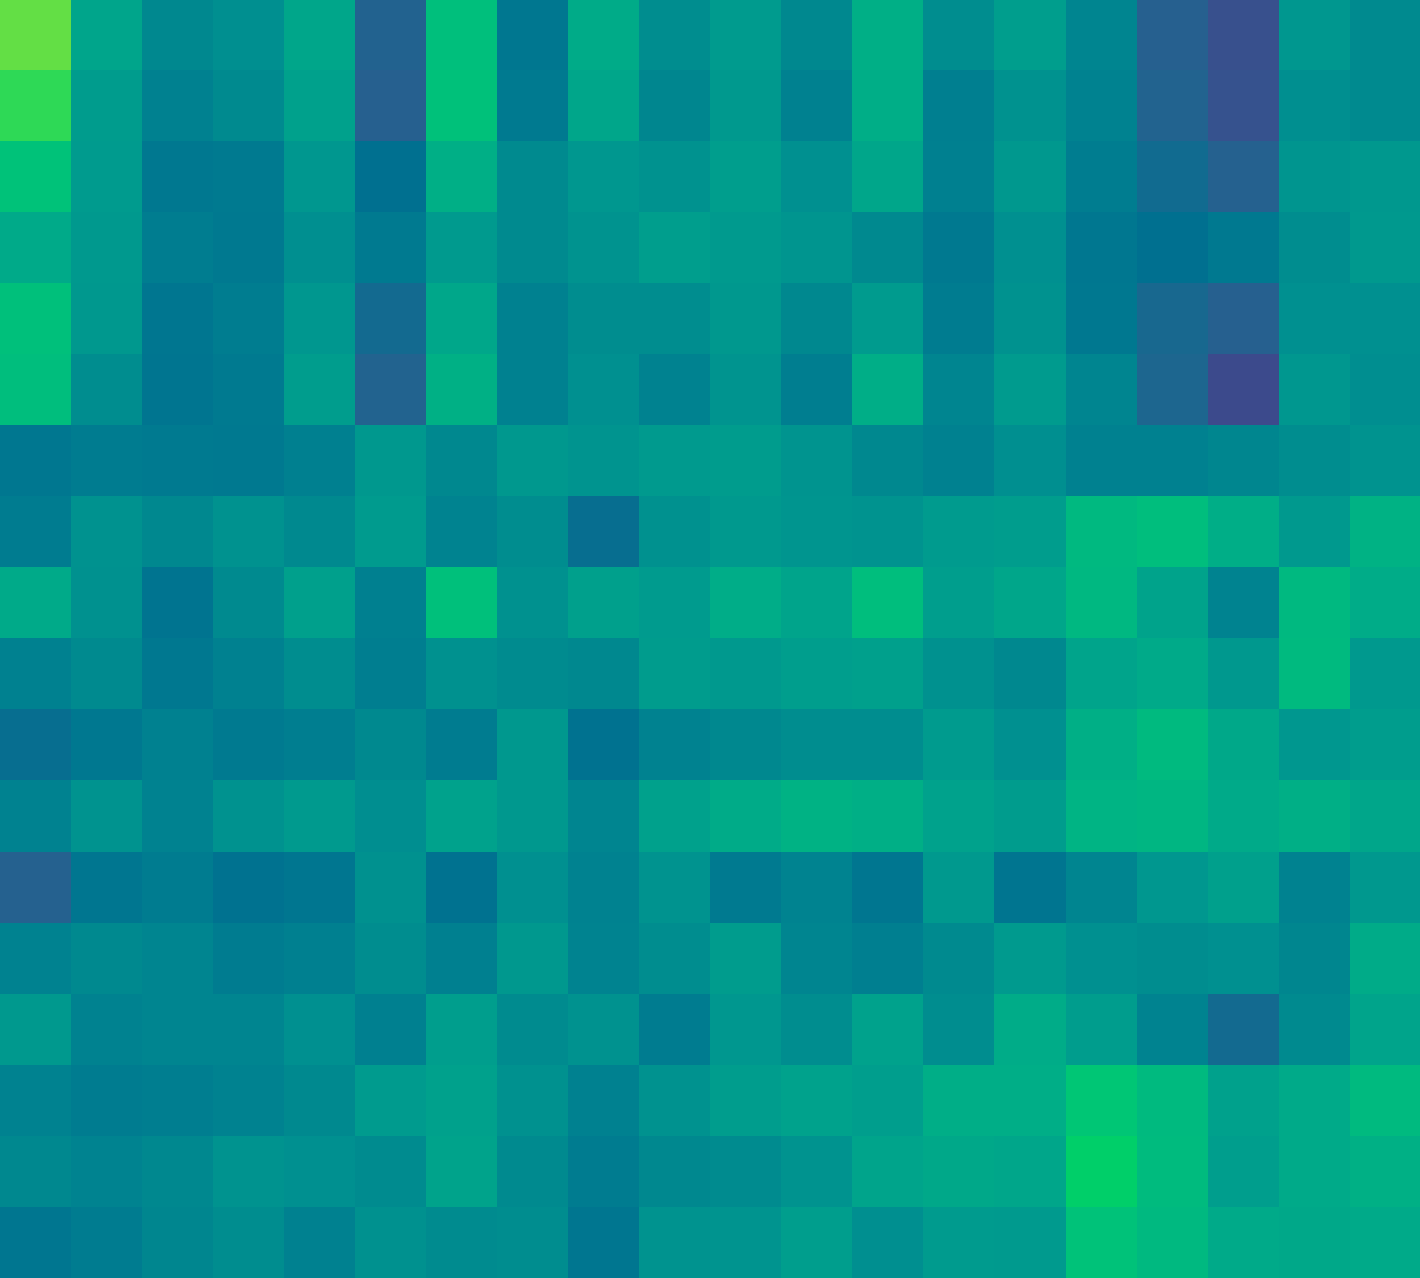
\includegraphics[height=1.8cm]{fig/matrices/b_tarrow}
		\vspace{-0.1\baselineskip}
		\caption{\centering R(2+1)D pre-trained on time arrow prediction}
	\end{subfigure}\hfill
	\begin{subfigure}[t]{0.5\linewidth}
		\centering\captionsetup{width=.9\linewidth, justification=raggedright}
		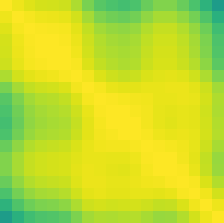
\includegraphics[height=1.8cm]{fig/matrices/a_vcop}
		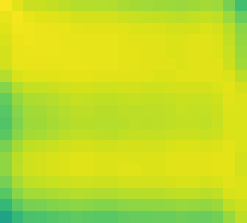
\includegraphics[height=1.8cm]{fig/matrices/b_vcop}
		\vspace{-0.1\baselineskip}
		\caption{\centering R(2+1)D pre-trained on clip order prediction}
	\end{subfigure}
	\par\medskip
	\begin{subfigure}[t]{0.5\linewidth}
		\centering\captionsetup{width=.9\linewidth, justification=raggedright}
		
\includegraphics[height=1.8cm]{fig/matrices/a_avg.png}
		
\includegraphics[height=1.8cm]{fig/matrices/b_avg.png}
		\vspace{-0.1\baselineskip}
		\caption{\centering Average pooling $1024$-dim embeddings}
	\end{subfigure}\hfill
	\begin{subfigure}[t]{0.5\linewidth}
		\centering\captionsetup{width=.9\linewidth, justification=raggedright}
		
\includegraphics[height=1.8cm]{fig/matrices/a_max.png}
		
\includegraphics[height=1.8cm]{fig/matrices/b_max.png}
		\vspace{-0.1\baselineskip}
		\caption{\centering Max pooling $1024$-dim embeddings}
	\end{subfigure}
	\par\medskip
	\begin{subfigure}[t]{0.5\linewidth}
		\captionsetup{width=.9\linewidth, justification=raggedright}
		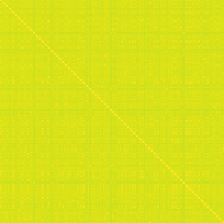
\includegraphics[height=1.8cm]{fig/matrices/a_amax.png}
		
\includegraphics[height=1.8cm]{fig/matrices/b_amax.png}
		\vspace{-0.1\baselineskip}
		\caption{\centering Argmax pooling $2048$-dim embeddings}
	\end{subfigure}\hfill
	\centering
	\par\medskip
	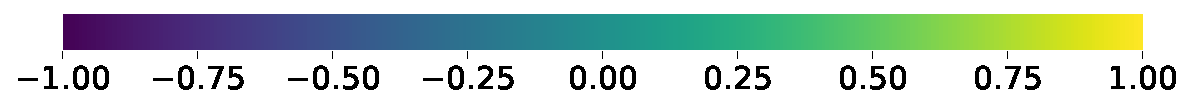
\includegraphics[width=0.48\textwidth]{fig/colorbar}
	\caption{Visualization of cosine similarities between different embeddings. For each pair, the left figure is matrix A and the right one is matrix B.}
	\label{fig:self_supervised_embeddings}
\end{figure}

%\begin{figure}[t]
%	\begin{subfigure}[t]{0.5\linewidth}
%		\centering\captionsetup{width=.9\linewidth, justification=raggedright}
%		
\includegraphics[height=1.8cm]{fig/matrices/a_avg.png}
%		
\includegraphics[height=1.8cm]{fig/matrices/b_avg.png}
%		\caption{\centering Average pooling $1024$-dim embeddings}
%	\end{subfigure}\hfill
%	\begin{subfigure}[t]{0.5\linewidth}
%		\centering\captionsetup{width=.9\linewidth, justification=raggedright}
%		
\includegraphics[height=1.8cm]{fig/matrices/a_max.png}
%		
\includegraphics[height=1.8cm]{fig/matrices/b_max.png}
%		\caption{\centering Max pooling $1024$-dim embeddings}
%	\end{subfigure}
%	\par\medskip
%	\centering
%	\begin{subfigure}[t]{0.5\linewidth}
%		\captionsetup{width=.9\linewidth, justification=raggedright}
%		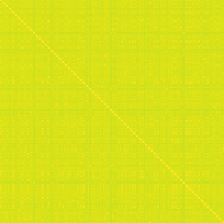
\includegraphics[height=1.8cm]{fig/matrices/a_amax.png}
%		
\includegraphics[height=1.8cm]{fig/matrices/b_amax.png}
%		\caption{\centering Argmax pooling $2048$-dim embeddings}
%	\end{subfigure}\hfill
%	\par\medskip
%	\centering
%	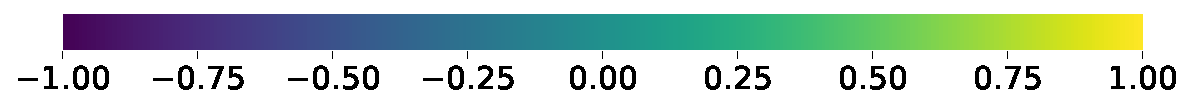
\includegraphics[width=0.48\textwidth]{fig/colorbar}
%	\caption{Visualization of cosine similarities between different DOPE-extracted embeddings. In the same fashion as in Figure \ref*{fig:self_supervised_embeddings}, for each pair, the left figure is matrix A and the right one is matrix B.}
%	\label{fig:DOPE_embeddings}
%\end{figure}

\subsection{Results on self-supervised features}
The results are summarized in Table \ref{tab:self-sup}. Unfortunately, the performance of embeddings obtained from R(2+1)D pre-trained on either Kinetics-400 or on self-supervised tasks do not come close to the baseline embeddings \cite{hmm}. We are disappointed by the fact that self-supervised training on PHOENIX-2014T does not improve upon Kinetics-400 features. We also downsampled the baseline embeddings by taking only 1 in 8 frames to match the number of embeddings that are output by R(2+1)D. The performance was only slightly worse.

\begin{table}[H]
	\centering
	\def\arraystretch{0.9}
	\setlength{\tabcolsep}{0.2em}
	\begin{tabular}{l c c}
		\toprule
		Input   & Our implem.   & Results from \cite{neccam} \\
		\midrule
		Gloss2Text   &  24.49 & 25.35 \\
		S2T, baseline \cite{hmm}   &  19.49 & 20.69  \\
		S2T, baseline \cite{hmm}, 1 in 8   &  17.08  &  -  \\
		S2T, kinetics R(2+1)D &  8.86 &  -  \\
		S2T, time arrow R(2+1)D  &  8.58 & - \\
		S2T, clip order R(2+1)D  &  8.41 & - \\
		\bottomrule
	\end{tabular}
	\vspace{-0.4\baselineskip}
	\caption{BLEU-4 on PHOENIX-2014T dev when training a Sign Language Transformer on self-supervised features. Note that in \cite{neccam}, the optimal number of beams and length penalty are grid-searched whereas we always take number of beams = 7 and length penalty = 1. }
	\label{tab:self-sup}
\end{table}


\subsection{Influence of Body Keypoints}

We summarize hereunder the translation performances observed on PHOENIX-2014T dev when feeding the network additionnal body keypoints inputs. Table \ref{tab:embeddings} shows the performances when concatenating the baseline embeddings \cite{neccam} with the pooled embeddings extracted from each video frame with DOPE.
\begin{table}[H]
\centering
\def\arraystretch{0.9}
\begin{tabular}{l c c c c}
	\toprule
	Input &  \multicolumn{4}{c}{DEV}\\
	\midrule
	{}   & BLEU-1   & BLEU-2    & BLEU-3   & BLEU-4\\
	baseline   &  45.54 & 32.60  & \textbf{25.30}  & \textbf{20.69}\\
	+avg   &  46.61 & 33.17   & 25.21  & 20.09\\
	+max   &  45.98  &  32.44   & 24.79  & 19.99\\
	+amax  &  \textbf{47.31} &  \textbf{33.34}   & 25.07  & 19.81\\
	+max+amax  &  44.32 & 31.50  & 24.09  & 19.27\\
	\bottomrule
\end{tabular}
\vspace{-0.4\baselineskip}
\caption{Sign2Text with additional Pooling Embeddings}
\label{tab:embeddings}
\end{table}
Table \ref{tab:2d_keypoints} (resp. Table \ref{tab:3d_keypoints}) shows the performances of the five best experiments obtained when concatenating the same baseline embeddings with the 2D (resp. 3D) body keypoints extracted using DOPE. 
\begin{table}[h]
	\centering
	\def\arraystretch{0.9}
	\begin{tabular}{l c c c c}
		\toprule
		Input &  \multicolumn{4}{c}{DEV}\\
		\midrule
		{}   & BLEU-1   & BLEU-2    & BLEU-3   & BLEU-4\\
		baseline  &  45.54 & \textbf{32.60}  & \textbf{25.30}  & \textbf{20.69}\\
		+hand\_2d   &  45.66 & 32.52   & 24.79  & 19.18\\
		+face\_2d   &  46.06  &  32.44   & 24.63  & 19.61\\
		+body\_2d   &  45.73 &  32.04   & 24.34  & 19.53\\	
		+fh\_2d\footnotemark[3]  &  45.53 &  32.21  & 24.31  & 19.34\\	
		+fhb\_2d\footnotemark[4] &  \textbf{46.09} &  32.16   & 23.96  & 18.75\\	
		\bottomrule
	\end{tabular}
	\vspace{-0.4\baselineskip}
	\caption{Sign2Text with additional 2D Keypoints}
	\label{tab:2d_keypoints}
\end{table}

\begin{table}[h]
	\centering
	\def\arraystretch{0.9}
	\begin{tabular}{l c c c c}
		\toprule
		Input &  \multicolumn{4}{c}{DEV}\\
		\midrule
		{}   & BLEU-1   & BLEU-2    & BLEU-3   & BLEU-4\\
		baseline  &  45.54 & 32.60  & \textbf{25.30}  & \textbf{20.69}\\
		+hand\_3d   &  46.19 & 32.49   & 24.24  & 18.92\\
		+face\_3d   &  45.56  &  32.10 & 24.27  & 19.27\\
		+body\_3d   &  44.96 &  31.96   & 24.32  & 19.46\\	
		+fh\_3d\footnotemark[3]  &  \textbf{46.37} &  \textbf{32.83}   & 24.88  & 19.72\\	
		+fhb\_3d\footnotemark[4]  &  46.09 &  32.34   & 24.00  & 18.85\\	
		\bottomrule
	\end{tabular}
	\vspace{-0.4\baselineskip}
	\caption{Sign2Text with additional 3D Keypoints}
	\label{tab:3d_keypoints}
\end{table}
\footnotetext[3]{face+hand keypoints} 
\footnotetext[4]{face+hand+body keypoints}

No matter what combination of additional inputs we feed the network, we do not witness any significative improvement in translation performances. This is mainly due to DOPE performing relatively poorly on the PHOENIX-2014T dev dataset. Even though it manages to identify body keypoints in almost every single frames, it only rarely detects the signer's face and hands (Figure \ref{fig:pie_charts}). Hence, we're mostly adding noise to the baseline embeddings. 
Instead of using a single model for whole-body pose estimation, one could try using indepedent hand, face and body experts to detect more precisely each part of the signer's expression. Multi-Channel Transformers \cite{multi-channel} were recently proposed to combine inputs from multiple such experts.

\begin{figure}[H]
	\centering
	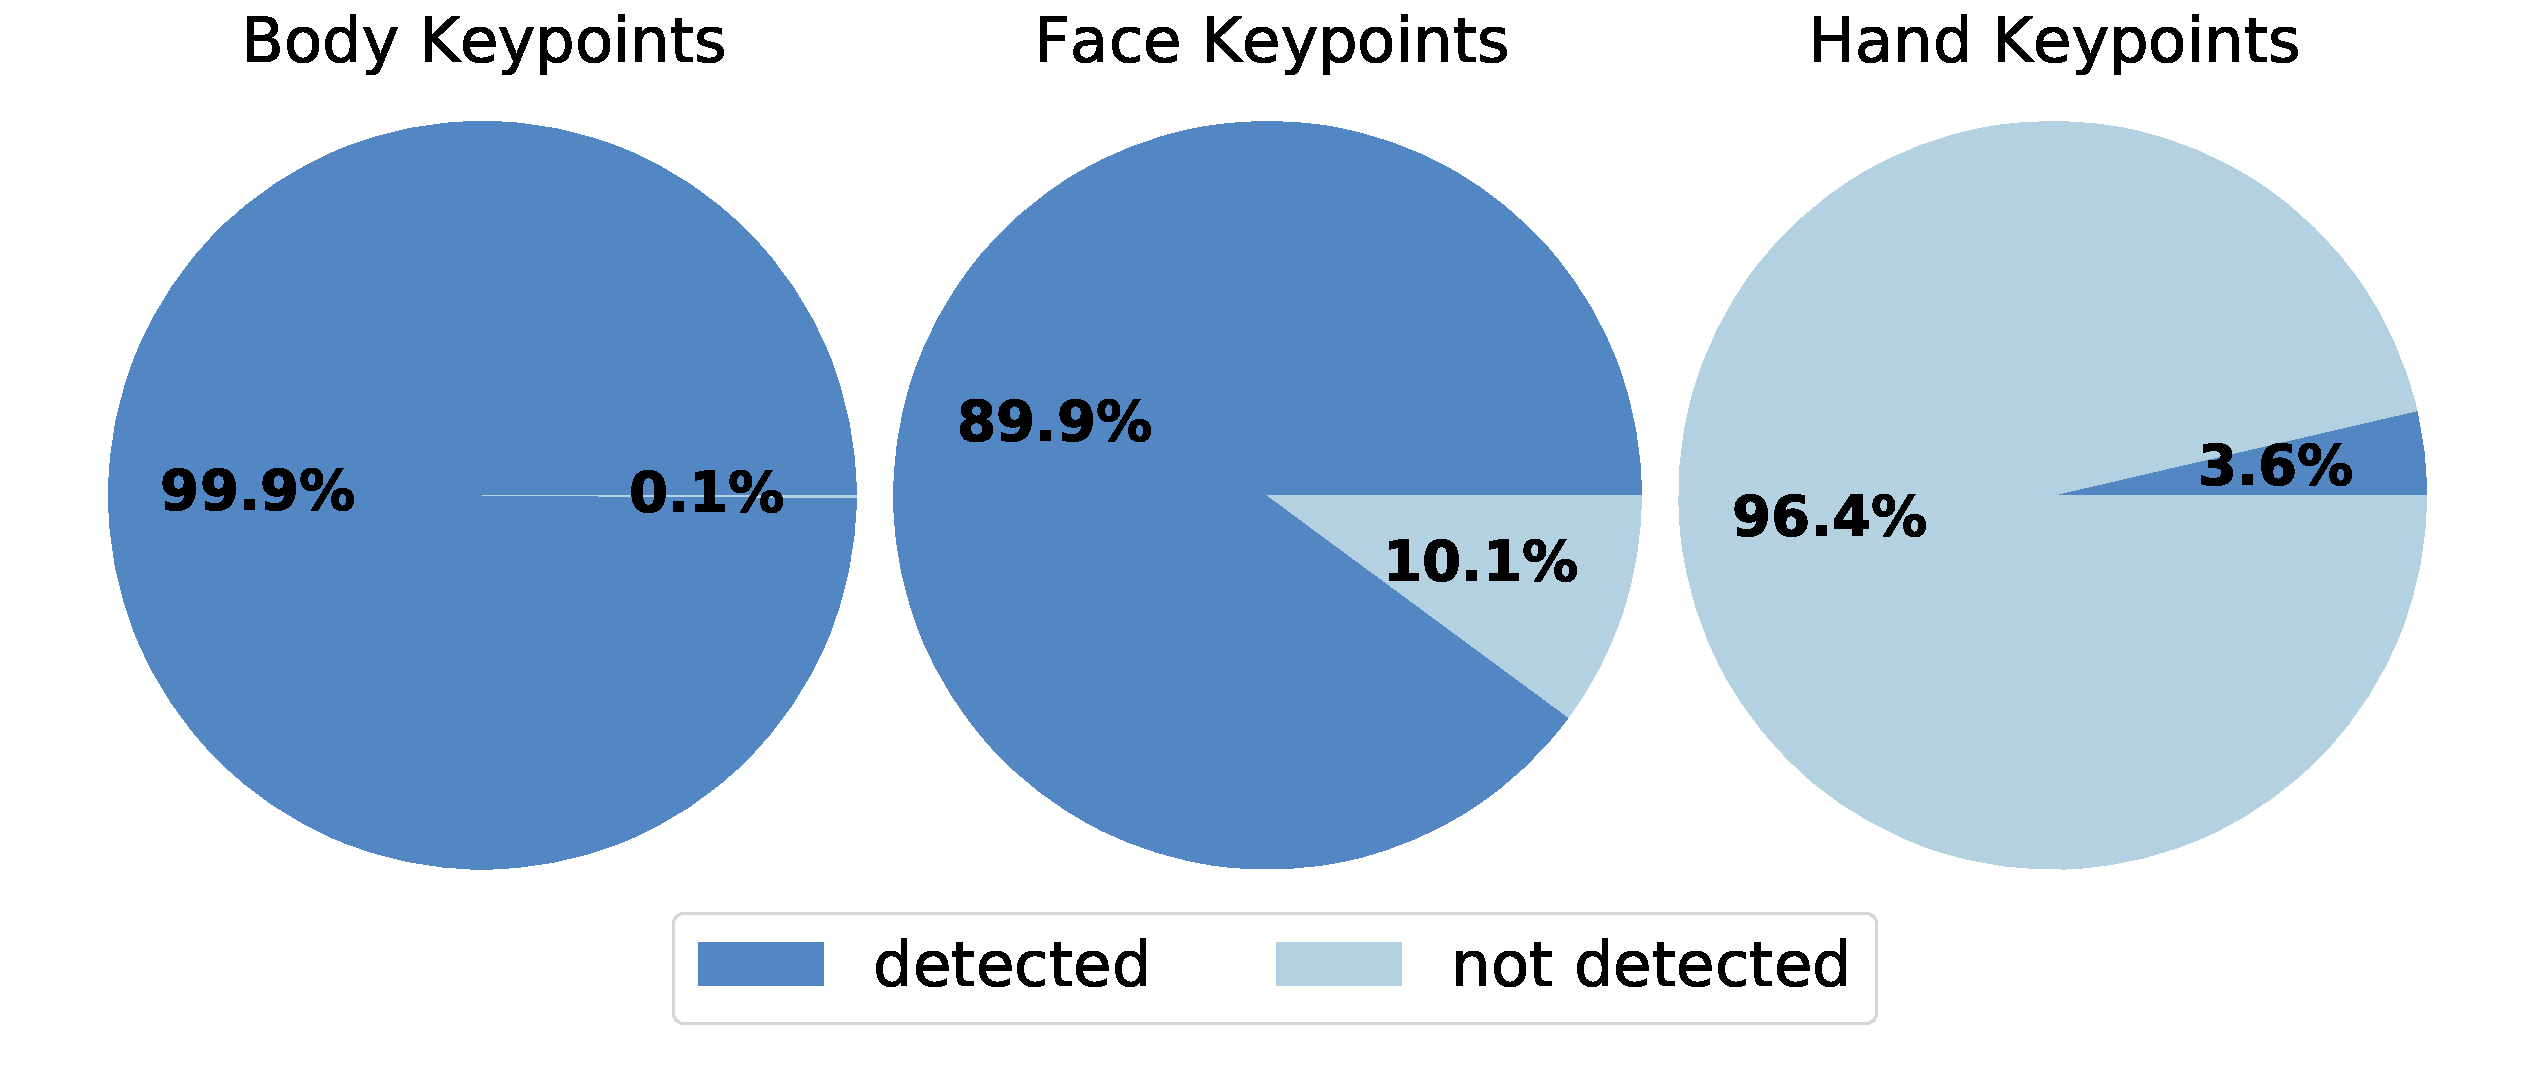
\includegraphics[width=8.7cm]{fig/keypoints.pdf}
	\vspace{-1.4\baselineskip}
	\caption{DOPE Results on  PHOENIX-2014T}
	\label{fig:pie_charts}
\end{figure} 


To further understand why DOPE-extracted body keypoints do not help improve the translation of our model, we plot the cosine similarities between the pooled embeddings of a given video with the pooled embeddings of the same video (matrix $A$) and with the pooled embeddings of another video (matrix $B$) (Figure \ref{fig:self_supervised_embeddings}). These matrices corroborate our findings: DOPE doesn't perform well on PHOENIX-2014T. Indeed, the pooled embeddings are highly similar because the model solely identifies the signer's body, which is nearly the same regardless of the video we are analyzing.
\section{Conclusion}
We explored two techniques for training a 3D feature extractor in a self-supervised way. While we did not obtain satisfying results, we still believe that self-supervised learning on larger datasets can be lead to improvements. Regarding the work done using humain body keypoints as additional inputs, we think that a more specialized pose estimation model is necessary in order to benefit sign language translation.


{\small
\bibliographystyle{ieee_fullname}
\bibliography{egbib}
}

\end{document}
